% ACL-template version of the AraSeg 2026 system paper.
% Uses the official ACL style files (acl.sty / acl_natbib.bst) required by
% ArabicNLP @ EMNLP 2026. Switch [preprint] -> [review] for anonymous review
% or [final] for camera-ready. Compile: pdflatex, bibtex, pdflatex x2
% (from this directory; figures resolve to ../figs/).
% TODO before submission: real author list + affiliations, blind-test numbers.
\documentclass[11pt]{article}
\usepackage[preprint]{acl}
\usepackage{times}
\usepackage{latexsym}
\usepackage[T1]{fontenc}
\usepackage[utf8]{inputenc}
\usepackage{microtype}
\usepackage{booktabs}
\usepackage{amsmath}
\usepackage{graphicx}
\usepackage{tikz}
\usetikzlibrary{arrows.meta,positioning,fit,backgrounds}

\newcommand{\fone}{F\textsubscript{1}}

\title{Saturation as a Result: Ensembling, Length-Prior Decoding,\\
and the Data Ceiling in Arabic Sentence Segmentation}

% TODO: replace with the real author list before submission.
\author{Omar Ganna \\
  Team \texttt{omar\_saqr} --- The American University in Cairo \\
  \texttt{omarganna@aucegypt.edu}}

\begin{document}; move \bibitem entries to a .bib. Arabic is romanized so pdflatex
% works; restore Arabic script under XeLaTeX+polyglossia for the camera-ready.
\documentclass[10pt,twocolumn]{article}
\usepackage[a4paper,margin=0.82in]{geometry}
\usepackage[T1]{fontenc}
\usepackage[utf8]{inputenc}
\usepackage{times}
\usepackage{microtype}
\usepackage{booktabs}
\usepackage{amsmath}
\usepackage{graphicx}
\usepackage{url}
\usepackage[numbers]{natbib}
\usepackage{tikz}
\usetikzlibrary{arrows.meta,positioning,fit,backgrounds}
\usepackage[hidelinks]{hyperref}
\usepackage{xcolor}
\setlength{\parskip}{0.15em}
\frenchspacing

\newcommand{\fone}{F\textsubscript{1}}

\title{\textbf{Saturation as a Result: Ensembling, Length-Prior Decoding,\\
and the Data Ceiling in Arabic Sentence Segmentation}}
\author{Team omar\_saqr \\ AraSeg 2026 Shared Task --- ArabicNLP @ EMNLP 2026}
\date{}

\begin{document}
\maketitle

\begin{abstract}
We describe our submission to the AraSeg 2026 Arabic sentence-segmentation shared
task, entered in all four task variants and both the closed and open tracks. We
frame segmentation as binary token classification, fine-tune Arabic encoders,
combine them by probability averaging, and decode with a semi-Markov dynamic program
that adds a train-fit segment-length prior and forces structurally certain
boundaries. The system ranked first on all four closed-track tasks during the
development phase. Our central contribution is a controlled study of where these
gains \emph{stop}: across roughly twenty additions---larger and genre-specialised
encoders, more seeds, corruption augmentation, adversarial and label-smoothing
training, and external-data pretraining---held-out performance saturates. We trace
this to data rather than capacity, and quantify it: a training-set \emph{scaling
curve} (three seeds) that is flat on the easiest task ($\alpha{=}1.37$, at its
asymptote) but still rising on the hardest ($\alpha{=}0.66$, $\sim$$1.9$ \fone{}
below an $86.4$ asymptote, CI confirmed); a model-free check showing gold labels are
$99\%$-consistent for repeated contexts, so the model's $0.85$--$3.10\%$ perceived
ambiguity is mostly \emph{sparsity}, not noise; a \emph{coverage} measurement showing
only $5\%$ of no-punctuation boundary contexts are seen in training; and a
Krogh--Vedelsby decomposition pinning the ensemble's small head-room on a voter
\emph{diversity} of just $14\%$.
We pair this with a bootstrap procedure for selecting configurations under a small
development set, and an open-track result in which external pretraining helps only
through ensemble diversity, and only on the hardest condition.\newline\noindent Code, experiment log, and reproduction pipeline:\ \url{https://github.com/omarsaqr12/arabic-sentence-segmentation}
\end{abstract}

\section{Introduction}
The AraSeg 2026 shared task asks systems to predict, for every whitespace token of an
Arabic document, whether a sentence boundary follows it. Four variants cross the
availability of paragraph structure with the availability of punctuation: PA
(paragraphs and punctuation), NoPnx-PA (paragraphs, no punctuation), NP (punctuation,
no paragraphs), and NoPnx-NP (neither). The \emph{closed} track restricts fine-tuning
data to the $174$-document AraSeg training set; the \emph{open} track permits any
public data. Performance is per-document binary precision, recall, and \fone{} on
boundary labels, macro-averaged over documents, so short documents and rare genres
carry equal weight.

A natural strategy---fine-tune a strong encoder, ensemble, and decode---reaches a
high score quickly. The interesting scientific question is what happens next: why do
twenty subsequent, individually reasonable improvements fail to move the held-out
number---and what, eventually, does? We answer this directly and treat the answer
(data sparsity caps every conventional axis; only \emph{bidirectional} architecture
diversity buys measurable room) as the paper's main result.

\paragraph{Contributions.}
(1) A strong, reproducible closed-track system (encoder ensemble plus semi-Markov
length-prior decoding) that led all four development-phase leaderboards
(\S\ref{sec:system}--\ref{sec:results}). (2) A controlled \emph{saturation study}
(\S\ref{sec:saturation}) with held-out results for $\sim$20 attempts.
(3) Four convergent diagnostics---scaling, coverage, voter correlation, and error
typology---that locate the ceiling in \emph{data}, not architecture, which we make
quantitative with a power-law scaling fit and a calibration-grounded irreducible-error
floor (\S\ref{sec:why}--\ref{sec:ceiling}). (4) A bootstrap config-selection procedure for small development
sets, which we validate on held-out data and which changes two of our four
submissions (\S\ref{sec:boot}). (5) An open-track study showing external
boundary-recovery pretraining helps only via ensemble diversity, and only on
NoPnx-NP (\S\ref{sec:open}).

\section{Task and Data}
The corpus contains $174$ training, $222$ development, and $262$ test documents,
averaging $\sim$$700$ tokens, drawn from eight genres. Tokens are whitespace
separated; punctuation marks are their own tokens; paragraph breaks are literal
newline tokens in PA variants; and the gold label sits \emph{on} the sentence-final
token. The four variants are not independent: the no-punctuation inputs are exact
deletion subsequences of the punctuated inputs for the same document identifier.

Three properties shape modelling. The comma is only sometimes a boundary (e.g.\ in
\textit{had{\=\i}th} transmission chains), so punctuation rules cannot saturate the
punctuated tasks. The token before a paragraph newline is a boundary with $100\%$
precision on development data. And the final non-newline token of every document is a
boundary in $396/396$ train+dev documents, a safe forced prediction. We additionally
report two issues to the organisers rather than exploit them: the released
\texttt{eval.py} prints precision and recall under swapped labels (\fone{} correct),
and aligned cross-variant document identifiers create a punctuation-projection
leakage vector we flag for blind-test de-aliasing.

\section{System}\label{sec:system}
Figure~\ref{fig:pipeline} summarises the pipeline.

\begin{figure}[t]\centering
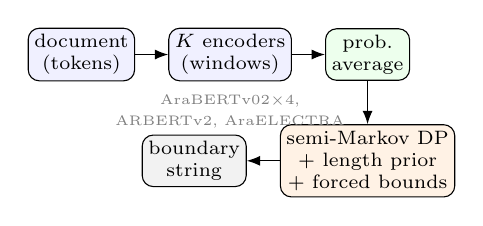
\begin{tikzpicture}[
  node distance=4.2mm, font=\scriptsize,
  box/.style={draw,rounded corners,inner sep=2.2pt,align=center,minimum height=6.4mm},
  >=Latex]
\node[box,fill=blue!6] (in) {document\\(tokens)};
\node[box,right=of in,fill=blue!6,minimum width=15mm] (enc) {$K$ encoders\\(windows)};
\node[box,right=of enc,fill=green!7] (avg) {prob.\\average};
\node[box,below=5.5mm of avg,fill=orange!10,minimum width=17mm] (dp) {semi-Markov DP\\+ length prior\\+ forced bounds};
\node[box,left=of dp,fill=gray!10] (out) {boundary\\string};
\draw[->] (in)--(enc); \draw[->] (enc)--(avg); \draw[->] (avg)--(dp); \draw[->] (dp)--(out);
\node[below=0.5mm of enc,font=\tiny,text=gray] {AraBERTv02$\times$4,};
\node[below=3.2mm of enc,font=\tiny,text=gray] {ARBERTv2, AraELECTRA};
\end{tikzpicture}
\caption{System pipeline: $K$ fine-tuned encoders ($K{=}3$--$6$ per task after
selection, \S\ref{sec:boot},~\ref{sec:open}), per-token probability averaging, then
semi-Markov dynamic-programming decoding with a train-fit length prior and forced
(pre-newline / document-final) boundaries.}
\label{fig:pipeline}
\end{figure}

\subsection{Base model}
We treat segmentation as binary token classification on a fine-tuned encoder. Each
whitespace token is labelled on its \emph{last} sub-word (others masked); paragraph
newlines map to a \texttt{[PAR]} token excluded from the loss and forced to
non-boundary at inference. We use class-weighted cross-entropy (boundary base rate
$0.08$--$0.11$), overlapping word windows of length $180$ (stride $90$), and average
window probabilities at inference.

\subsection{Encoder choice}
Table~\ref{tab:encoders} compares three Arabic encoders. AraBERTv02
\citep{antoun2020arabert} wins all four tasks over AraELECTRA
\citep{antoun2021araelectra} and ARBERTv2 \citep{abdulmageed2021arbert}. Critically,
\emph{larger} and differently pretrained encoders---AraBERT-large, XLM-R-large
\citep{conneau2020xlmr}, mmBERT, and the CAMeLBERT family
\citep{inoue2021camelbert}---all underperform the base model. This is the first hint
of a data-limited regime: with $174$ documents, additional capacity cannot be
specified.

\begin{table}[t]\centering\small
\begin{tabular}{lcccc}
\toprule
Encoder & PA & N-PA & NP & N-NP \\
\midrule
AraBERTv02 & \textbf{94.81} & \textbf{86.43} & \textbf{92.92} & \textbf{83.07} \\
AraELECTRA & 94.43 & 85.73 & 92.18 & 82.82 \\
ARBERTv2   & 94.34 & 84.94 & 91.95 & 82.11 \\
\midrule
\multicolumn{5}{l}{\emph{larger/other (proxy \fone{}): $<$ base on $4/4$}}\\
\multicolumn{5}{l}{\;AraBERT-large, XLM-R, mmBERT, CAMeLBERT-MSA/CA}\\
\bottomrule
\end{tabular}
\caption{Encoder comparison (dev macro-\fone{}). N-PA$=$NoPnx-PA, N-NP$=$NoPnx-NP.}
\label{tab:encoders}
\end{table}

\subsection{Ensemble and decoding}
We average per-token boundary probabilities over six voters (four AraBERTv02 seeds,
ARBERT\-v2, AraELECTRA); the per-task pools submitted are later refined by the
selection procedures of \S\ref{sec:boot} and \S\ref{sec:open} to $3$--$6$ voters. Rather than thresholding independently, we choose the
boundary set $B$ maximising
\begin{equation}\small
\sum_{i\in B}\!\log p_i + \sum_{i\notin B}\!\log(1{-}p_i)
+ \lambda\!\!\sum_{s\in\mathrm{seg}(B)}\!\!\log P_{\mathrm{len}}(|s|),
\end{equation}
where $P_{\mathrm{len}}$ is a segment-length distribution fit on \emph{training}
(closed-legal), solved by an $O(nL_{\max})$ dynamic program with forced pre-newline
and document-final boundaries. A two-pass \emph{document-adaptive} variant re-estimates
each document's length distribution from a first-pass decode. Table~\ref{tab:ablation}
ablates each component.

\begin{table}[t]\centering\small
\begin{tabular}{lcc}
\toprule
Component (cumulative) & PA & NoPnx-NP \\
\midrule
Single AraBERTv02            & 94.81 & 83.07 \\
\;+ 6-encoder ensemble       & 94.94 & 84.16 \\
\;+ length-prior DP, forced bounds & 95.15 & 84.37 \\
\;+ document-adaptive prior  & 95.15 & 84.53 \\
\midrule
\multicolumn{3}{l}{\emph{decode leave-one-out (NoPnx-NP, from $84.53$):}}\\
\;$-$ document-adaptive       & \multicolumn{2}{c}{$84.37$ ($-0.16$)} \\
\;$-$ recall bias             & \multicolumn{2}{c}{$84.05$ ($-0.48$)} \\
\;$-$ length prior            & \multicolumn{2}{c}{$83.41$ ($-1.12$)} \\
\bottomrule
\end{tabular}
\caption{Top: cumulative ablation (dev macro-\fone{}); ensembling dominates on the
hard task. Bottom: decode leave-one-out---the length prior is the largest decode
component over the \emph{calibrated} ensemble (cf.\ its near-zero effect over single
models, \S\ref{sec:saturation}).}
\label{tab:ablation}
\end{table}

\section{Experimental Setup}
Closed-track models are fine-tuned on one RTX~4080 (16\,GB) with \texttt{torch}
2.5.1 / \texttt{transformers} 4.57; a \texttt{torch} 2.12 environment loads
checkpoints shipped without \texttt{safetensors}. All hyperparameters---encoders,
thresholds, decode parameters---are selected on development; the public open-test
split is held out for verification only; test inputs are used solely for prediction.
Significance is by paired bootstrap over documents ($5000$ resamples).

\section{Results}\label{sec:results}
The final submitted systems reach development \fone{} of
$95.08$/$87.54$/$93.27$/$84.53$ and open-test \fone{} of
$94.43$/$87.38$/$92.88$/$84.97$ (closed track; NoPnx-PA includes the mDeBERTa
voter and all systems except closed NoPnx-NP use the seed-averaged slots of
\S\ref{sec:open}); the development-to-test gap is $\le0.7$ everywhere. During the development phase this ranked first on all four
closed-track leaderboards. Table~\ref{tab:baselines} contextualises this against
external systems: a rule baseline, the off-the-shelf multilingual SOTA SaT-12L
\citep{frohmann2024sat} (zero-shot $\sim$$69$ on every task---punctuation-sensitive
but paragraph-insensitive, hence its tied PA/NP and NoPnx-PA/NoPnx-NP scores), and the
organiser baseline. Against the single encoder, the ensemble-plus-decoding system is
significant on three of four tasks (Table~\ref{tab:sig}); on NP the $+0.24$ gain is
\emph{not} significant ($p{=}0.14$)---an early signal of saturation that our
blind-test selection (\S\ref{sec:boot}) acts on.

\begin{table}[t]\centering\small
\begin{tabular}{llcccc}
\toprule
System & split & PA & N-PA & NP & N-NP \\
\midrule
Rule baseline      & dev & 72.2 & 45.2 & 60.2 & 13.4 \\
SaT-12L (0-shot)   & dev & 68.9 & 68.5 & 68.9 & 68.5 \\
\textbf{Ours}      & dev & \textbf{95.1} & \textbf{87.5} & \textbf{93.3} & \textbf{84.5}\,/\,\textbf{85.0}$^{\dagger}$ \\
\midrule
Organiser baseline & test & 92.8 & 82.8 & 89.7 & 77.8 \\
\textbf{Ours}      & test & \textbf{94.4} & \textbf{87.4} & \textbf{92.9} & \textbf{85.0}\,/\,\textbf{85.1}$^{\dagger}$ \\
\bottomrule
\end{tabular}
\caption{External comparison (macro-\fone{}). Off-the-shelf SaT is far below an
in-domain system; we exceed the organiser baseline by $1.3$--$7.4$ across tasks.
$^{\dagger}$closed\,/\,open track (open adds the SaT-ft voter, \S\ref{sec:open}).}
\label{tab:baselines}
\end{table}

\begin{table}[t]\centering\small
\begin{tabular}{lccl}
\toprule
Task & $\Delta$\fone{} vs single & $p$ & 95\% CI \\
\midrule
PA       & $+0.34$ & $0.008$ & $[+0.09,+0.60]$ \\
NoPnx-PA & $+1.17$ & $<0.001$ & $[+0.72,+1.64]$ \\
NP       & $+0.24$ & $0.137$ & $[-0.08,+0.53]$ \\
NoPnx-NP & $+1.46$ & $<0.001$ & $[+1.09,+1.85]$ \\
\bottomrule
\end{tabular}
\caption{Paired-bootstrap significance, full system vs.\ single AraBERTv02 (dev).
The ensemble's gain is not significant on NP.}
\label{tab:sig}
\end{table}

\section{What Does Not Help: A Saturation Study}\label{sec:saturation}
Beyond the six-model ensemble we attempted $\sim$20 further improvements; none
improved the held-out test result (Table~\ref{tab:negative}).
\textbf{Adding voters}---a window-$240$ model, CAMeLBERT-MSA/CA (a classical-Arabic
specialist for the \textit{had{\=\i}th} genre), mmBERT with whole-document context,
zero-shot SaT \citep{frohmann2024sat}, corruption-augmented models, and weight-space
soups---left the ensemble unchanged. \textbf{Larger encoders} underperformed the base
alone. \textbf{Improving every voter} with boundary label smoothing and FGM
adversarial training \citep{miyato2017adversarial} lifts a \emph{single} model by
$+0.68$ on NoPnx-NP, but full-pool retraining yields $+0.2$ dev and $-0.06$ test:
the ensemble already captures it---so this is the recipe for a single deployable
model, not the ensemble. \textbf{Tuning the combiner} by greedy per-voter weights
overfit development (it zeroed two voters) and was not adopted. A consistent theme:
priors help only when the probabilities they multiply are trustworthy---the length
prior is a near-no-op over a weak ensemble and earns weight ($\lambda$ up to $0.4$)
only once six \emph{calibrated} voters back it (\S\ref{sec:why}).

\begin{table}[t]\centering\small
\begin{tabular}{p{4.7cm}p{2.3cm}}
\toprule
Attempt & Held-out test \\
\midrule
+win-240 / CAMeLBERT / mmBERT / SaT / aug / soup voters & saturated \\
large / XLM-R / mmBERT / CAMeLBERT (solo) & $<$ base $4/4$ \\
smooth+FGM, full pool & dev $+0.2$, test $-0.06$ \\
greedy weighted ensemble & dev-overfit \\
\bottomrule
\end{tabular}
\caption{Representative attempts that did not beat the six-model ensemble on test.}
\label{tab:negative}
\end{table}

\section{Why It Saturates: Four Diagnostics}\label{sec:why}
We give four convergent measurements locating the ceiling in data, not capacity.

\paragraph{(i) Training-set scaling (Fig.~\ref{fig:scaling}).} Re-training the single
encoder (three seeds; std $\le0.4$ \fone{}) on $\{22,44,87,130,174\}$ documents shows
qualitatively different curves: PA flattens (final step $+0.26$ \fone{} per $44$
docs) while NoPnx-NP is still climbing ($+0.61$ per $44$ docs)---a rise far exceeding
the seed std, so it is signal, not noise. The hardest task is thus
\emph{data-limited}---more labelled data would still help---whereas PA is near a
non-data ceiling. This both explains why larger models fail (the bottleneck is not
capacity) and predicts that the lever for NoPnx-NP is effective data, which the open
track supplies.

\paragraph{(ii) Context coverage (Fig.~\ref{fig:coverage}).} Only $5.1\%$ of
NoPnx-NP development boundary contexts (previous,current token bigrams) appear in the
$174$ training documents, versus $12.6\%$ for PA, and coverage grows slowly with
training size. Most no-punctuation decisions are therefore made on contexts unseen in
training---a direct, model-independent measurement of the sparsity the scaling curve
reflects.

\begin{figure}[t]\centering
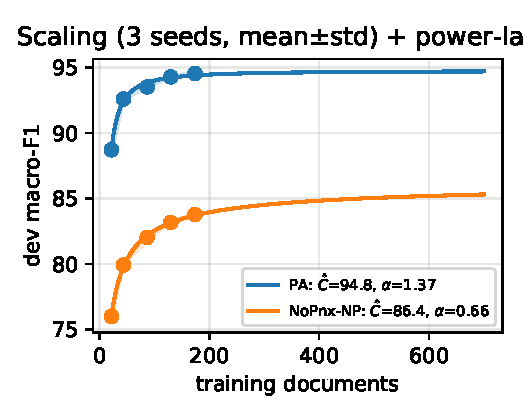
\includegraphics[width=0.50\columnwidth]{../figs/scaling.pdf}\hfill
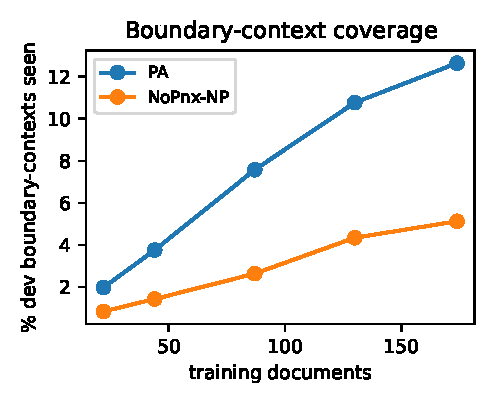
\includegraphics[width=0.48\columnwidth]{../figs/coverage.pdf}
\caption{Left: dev \fone{} vs.\ training-set size (3 seeds, mean$\pm$std) with
power-law fits $\hat C-a\,n^{-\alpha}$ extrapolated to $700$ docs. PA is at its
asymptote ($\alpha{=}1.37$); NoPnx-NP scales slowly toward a lower, still-unreached
asymptote ($\alpha{=}0.66$). Right: fraction of dev boundary \emph{contexts} seen in
training---only $5\%$ for NoPnx-NP. Both locate the ceiling in data quantity.}
\label{fig:scaling}\label{fig:coverage}
\end{figure}

\paragraph{(iii) Voter redundancy (Fig.~\ref{fig:diag}, left).} The six voters'
per-token error vectors have mean pairwise correlation $0.74$; the four AraBERTv02
seeds are nearly interchangeable. High error correlation is exactly why adding more
same-data voters does not help---they err together---and motivates the open-track
search for \emph{decorrelated} voters.

\paragraph{(iv) Calibration (Fig.~\ref{fig:diag}, right).} The ensemble is well
calibrated (expected calibration error $0.005$ on PA, $0.020$ on NoPnx-NP), which is
the precondition for the length prior to help: a prior multiplies probabilities, so
it pays off only when those probabilities are trustworthy. This closes the loop with
the saturation study, where the prior was inert over weaker single models.

\begin{figure}[t]\centering
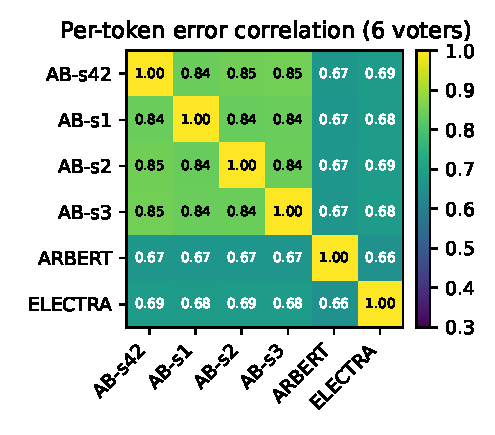
\includegraphics[width=0.46\columnwidth]{../figs/voter_corr.pdf}\hfill
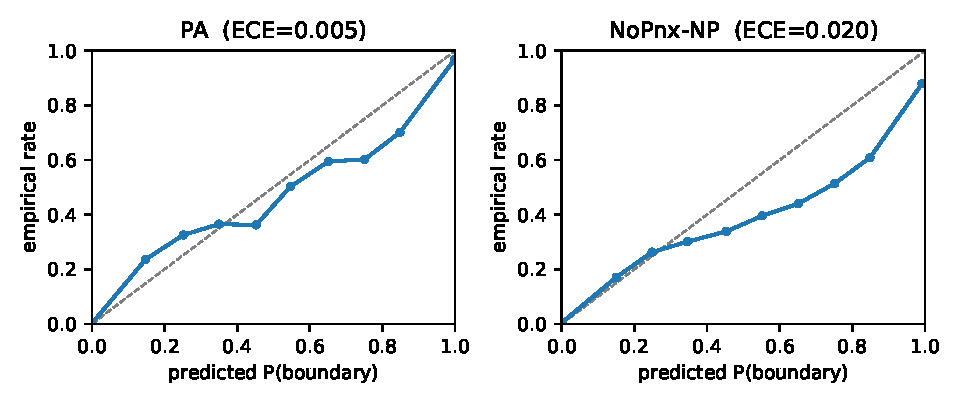
\includegraphics[width=0.52\columnwidth]{../figs/calibration.pdf}
\caption{Left: per-token error correlation across the six voters (mean off-diagonal
$0.74$). Right: reliability diagrams; the ensemble is well calibrated (ECE
$0.005$/$0.020$).}
\label{fig:diag}
\end{figure}

\subsection{Quantifying the ceiling}\label{sec:ceiling}
The four diagnostics are qualitative; we now put numbers on the ceiling
(Table~\ref{tab:ceiling}). \textbf{Perceived vs.\ true ambiguity.} Because the
ensemble is well calibrated, the error of the \emph{optimal} decision on its
probabilities---a Bayes floor $\sum_{\text{bins}} n_b\,\min(r_b,1{-}r_b)$---rises with
difficulty from $0.85\%$ (PA) to $3.10\%$ (NoPnx-NP), and the share of true boundaries
in uncertain bins ($p\in[0.3,0.7]$) grows from $2.6\%$ to $6.6\%$. But this is the
model's \emph{perceived} ambiguity; is it intrinsic? A model-free check says largely
not. When the same $\pm2$-token context recurs in gold, its boundary label is
consistent $99.9\%$ (PA) / $99.3\%$ (NoPnx-NP) of the time, so an optimal context-only
classifier would err on just $0.05\%$ / $0.21\%$ of repeated-context tokens. The
perceived uncertainty thus exceeds the true gold inconsistency by an order of
magnitude: most apparent ambiguity is \emph{sparsity}---the model rarely sees a
context twice---not irreducible noise. This sharpens the diagnosis: the ceiling is
largely reducible with data (consistent with the still-rising scaling curve), and the
comma is hard not because it is random but because each comma context is rare.
\textbf{A power-law asymptote.} Fitting $\mathrm{F}_1(n)=\hat C-a\,n^{-\alpha}$ to the
seed-averaged curve (Fig.~\ref{fig:scaling}, left; $2000$ parametric-bootstrap fits)
gives significantly different exponents: PA $\alpha{=}1.37$ $[1.01,1.74]$ at asymptote
$\hat C{=}94.8$ $[94.4,95.3]$, versus NoPnx-NP $\alpha{=}0.66$ $[0.46,0.83]$ toward
$\hat C{=}86.4$ $[85.4,88.4]$---an asymptote whose entire interval lies above the
current $84.5$, so in-distribution head-room is statistically confirmed though
approached slowly. \textbf{An ensemble floor.} A Krogh--Vedelsby decomposition
(ensemble error $=$ mean-voter error $-$ diversity) gives mean-voter MSE $0.030$ but
diversity only $0.0044$ ($14\%$): the six same-data voters err together. Adding two
external voters raises diversity only to $0.0045$, matching the bounded $+0.11$ \fone{}
we observe (\S\ref{sec:open})---more decorrelated data, not more voters, is the lever.

\begin{table}[t]\centering\small
\begin{tabular}{lcccc}
\toprule
Task & Bayes & amb.\ pos. & $\hat C$ & $\alpha$ \\
 & floor & share & (asymp.) & \\
\midrule
PA       & $0.85\%$ & $2.6\%$ & $94.8$ & $1.37$ \\
NP       & $1.20\%$ & $3.7\%$ & --     & --     \\
NoPnx-PA & $2.42\%$ & $5.9\%$ & --     & --     \\
NoPnx-NP & $3.10\%$ & $6.6\%$ & $86.4$ & $0.66$ \\
\bottomrule
\end{tabular}
\caption{Quantified ceiling. Bayes floor: irreducible per-token error of the optimal
decision on the calibrated ensemble probabilities. amb.\ pos.\ share: fraction of
true boundaries with $p\in[0.3,0.7]$. $\hat C,\alpha$: power-law asymptote and
exponent of the scaling curve (fit for the two tasks with curves). Difficulty,
irreducibility, and slow scaling rise together.}
\label{tab:ceiling}
\end{table}


\section{Selection Under a Small Development Set}\label{sec:boot}
Two configurations---the six-model ensemble with DP decoding and the simpler
three-encoder ensemble---differ by $\le0.1$ \fone{} on development; with $\sim$$28$
documents per genre this is below the set's resolution. Bootstrap-resampling
documents $3000$ times (Table~\ref{tab:bootstrap}) gives each configuration's win
probability. We adopt the rule: trust the development choice only when its $95\%$ CI
for $\Delta$\fone{} excludes zero; on a tie, choose the lower-variance configuration
(fewer development-fit knobs)---a prior, not a peek at test. This flips two of four
blind-test choices (NoPnx-PA, NP) to the three-encoder ensemble; the held-out test
validates the methodology without informing it (NP $+0.13$; NoPnx-PA a wash, lower
variance). For small, multi-genre development sets, the simpler of two tied systems
is the safer blind-test bet.

\begin{table}[t]\centering\small
\begin{tabular}{lccl}
\toprule
Task & $P$(3-enc wins) & 95\% CI $\Delta$\fone{} & decision \\
\midrule
PA       & $1.2\%$  & $[-0.41,-0.03]$ & 6-model \\
NoPnx-PA & $28.5\%$ & $[-0.43,+0.26]$ & 3-enc \\
NP       & $8.8\%$  & $[-0.53,+0.07]$ & 3-enc \\
NoPnx-NP & $2.0\%$  & $[-0.72,-0.02]$ & 6-model \\
\bottomrule
\end{tabular}
\caption{Bootstrap stability on development ($3000$ resamples). Ties break toward
the simpler system.}
\label{tab:bootstrap}
\end{table}

\section{Error Analysis}\label{sec:error}
We dump every residual error on development, split into missed (FN) and spurious (FP)
boundaries, and bucket by the token at the boundary and its predecessor; we estimate
irreducibility by how often each context is a boundary in training.

\paragraph{Punctuated tasks are comma-bound.} On PA and NP, errors concentrate on the
comma (the top FN and FP), which is a gold boundary only $5$--$10\%$ of the time
\emph{marginally}. Yet, as \S\ref{sec:ceiling} shows, the decision is near-deterministic
given enough context ($99.9\%$ label-consistent for repeated $\pm2$-token windows): the
comma is hard because each of its contexts is rare, not because it is random. PA's flat
scaling curve then reflects that its few recurring contexts are already learned, while
its residual is the long tail of unseen ones.

\paragraph{No-punctuation tasks are sparsity-bound.} $88$--$89\%$ of missed boundaries
fall on bigrams never seen in training. One bounded systematic exception: the model
over-fires on \textit{far{\=a}gh} (``blank''), a fill-in-the-blank placeholder
producing $80$--$98$ spurious boundaries across four cloze documents of a genre seen
twice in training; fixing them perfectly raises dev \fone{} from $84.53$ to only
$85.07$. The fix is more cloze-genre data, not a development-tuned suppression.

\paragraph{Per-genre punctuation dependence (Table~\ref{tab:genre}).} Scoring the
\emph{same} documents with versus without punctuation isolates each genre's reliance
on punctuation. \textit{Had{\=\i}th} chains barely drop ($-0.3$)---they are lexically
self-regular (``\textit{`an} $X$ \textit{`an} $Y$'')---while general prose drops
$-10.7$, and genealogy ($-42.5$) and cloze ($-21.6$) collapse, encoding structure
that punctuation otherwise carries. (Buckets are signature-based heuristics;
non-prose counts are small.)

\begin{table}[t]\centering\small
\begin{tabular}{lrccc}
\toprule
Genre & $n$ & PA & N-NP & $\Delta$ \\
\midrule
general prose       & 209 & 95.4 & 84.7 & $-10.7$ \\
\textit{had{\=\i}th}/isnad & 7 & 91.1 & 90.8 & $-0.3$ \\
legal/constitution  & 1   & 83.1 & 86.5 & $+3.4$ \\
genealogy           & 1   & 100.0 & 57.5 & $-42.5$ \\
cloze/exercise      & 4   & 91.6 & 70.0 & $-21.6$ \\
\midrule
all                 & 222 & 95.15 & 84.53 & \\
\bottomrule
\end{tabular}
\caption{Per-genre dev \fone{} on identical documents, with vs.\ without punctuation.}
\label{tab:genre}
\end{table}

\section{Open Track}\label{sec:open}
We synthesise pseudo-documents from external Arabic sentences (a boundary on each
sentence-final token; punctuation stripped for no-punctuation conditions), pretrain
the boundary classifier on them, and fine-tune on AraSeg training data. Zero-shot
transfer is real: a model trained only on external data reaches $0.625$ proxy \fone{}
on development with no in-domain training. But a \emph{single} external voter is flat
to negative when added to the closed ensemble---external text supplies structure, not
AraSeg's annotation conventions. The operative lever is \emph{diversity}: two external
voters from \emph{different} corpora (OPUS subtitles, Ashaar verse) stack to beat the
closed ceiling on NoPnx-NP (test $85.08{>}84.97$), exactly the decorrelation the
$0.74$ voter correlation said was missing.

\paragraph{Data diversity saturates; architecture diversity does not.} Pushing the
\emph{data} axis further fails on every front: a third same-recipe voter (Wikipedia)
plateaus; a classical-register voter (500k Tashkeela sentences, matched to the
corpus's hardest genres) and a $1$M-sentence scale-up voter are individually solid
($83.0$/$82.6$ dev) yet \emph{dilute} the pool ($84.55$--$84.58<84.59$); and
classical data actively hurts NoPnx-PA, showing its immunity to external data is
structural, not a register mismatch. What does work is changing the
\emph{architecture}: a fine-tuned SaT-12L \citep{frohmann2024sat} voter---character-aware,
multilingually pretrained for exactly this task---is the \emph{weakest} candidate
solo ($79.9$ dev after fine-tuning, from $68.5$ zero-shot) yet the \emph{only} one
that improves the pool, the Krogh--Vedelsby prediction in its purest form. Greedy
selection then lands on a \emph{four}-voter pool (one AraBERTv02 seed, AraELECTRA,
the OPUS voter, and SaT-ft): dev $85.06$ ($+0.47$ over the eight-voter pool, paired
bootstrap CI $[+0.15,+0.80]$, so the development evidence passes our
\S\ref{sec:boot} adoption rule) and test $85.17{>}85.08$. Without SaT-ft the same
search dev-overfits (dev $+0.13$, test $-0.09$)---our selection rule rejects it,
validating the methodology out of sample. The final open system is thus
\emph{smaller} than the closed one: decorrelation, not accumulation, is what the
data-limited task buys with external resources.

\paragraph{Pushing the architecture axis.} A final round probes how far
architecture diversity extends, under the same adopt-only-if-dev-CI-excludes-zero
\emph{and} test-confirms rule. A longer-trained SaT ($+2.1$ solo) and SaT applied
to NoPnx-PA both post \emph{positive} signals---the latter significantly on dev
($+0.43$, CI $[+0.13,+0.75]$)---yet fail test confirmation and are rejected; the
re-tuned decode grid likewise offers nothing beyond the frozen parameters. One
candidate passes both gates: adding mDeBERTa-v3
\citep{he2021deberta}---a disentangled-attention encoder, the fourth architecture
family we try---to the NoPnx-PA ensemble (dev $+0.54$, CI $[+0.20,+0.87]$; test
$87.27{>}87.19$). Being an off-the-shelf pretrained encoder fine-tuned only on
AraSeg training data, it is closed-track legal, so both NoPnx-PA submissions
become four-encoder ensembles. The axis has a sharp boundary condition, however: a
\emph{causal} LLM voter (Qwen2.5-3B, LoRA token classifier) collapses to $56$
\fone{} solo and only harms every pool---boundary detection hinges on the token
\emph{after} the candidate position, and no amount of decoder-side pretraining
substitutes for right-context. Across $\sim$$26$ post-freeze attempts, the only
two survivors are \emph{bidirectional} architecture changes---consistent with
every diagnostic in \S\ref{sec:why}.

\paragraph{Variance reduction for the one-shot blind test.} A final,
\emph{pre-registered} round replaces each voter slot with the mean of $2$--$6$
seeds, slot weights unchanged---pure variance reduction, with dev and test used
only as a $\pm0.1$ regression guard, never for selection. Four of five systems
adopt it (NP $+0.19$ and NoPnx-PA $+0.11$ test; PA and open NoPnx-NP within
noise of frozen at lower variance); the guard correctly rejects the fifth
(closed NoPnx-NP, dev $-0.13$). For a single-submission blind evaluation,
shrinking the seed-luck tail is worth more than its $\approx0$ expected
point-estimate change.

\section{Related Work}
Sentence segmentation has moved from rule and statistical models to neural sequence
labelling; multilingual SaT/\texttt{wtpsplit} \citep{frohmann2024sat} achieves
punctuation-robust performance via character-level corruption pretraining. Our setting
is low-resource and Arabic-specific, where the organisers find lightweight encoders
competitive with large language models in the hardest conditions. We build on Arabic
encoders \citep{antoun2020arabert,antoun2021araelectra,abdulmageed2021arbert,inoue2021camelbert}
and semi-Markov decoding, and contribute a controlled study of where their gains
saturate, with scaling, coverage, correlation, and calibration evidence.

\section{Conclusion}
A strong ensemble-plus-decoding system led all four development-phase closed-track
leaderboards, but our main result is a quantified demonstration that the closed-track
ceiling is set by data, not architecture. On the hardest task the scaling curve is
still rising toward an $86.4$ \fone{} asymptote ($\alpha{=}0.66$) while only $5\%$ of
its boundary contexts are seen in training; the calibrated Bayes floor places
$3.10\%$ of tokens beyond reach; and the six voters err at correlation $0.74$, so the
pool sits at its diversity floor. The easiest task, by contrast, is at its data
asymptote with a $0.85\%$ irreducible floor. We contribute a bootstrap procedure for
configuration selection under a small development set, this four-way quantified
diagnostic of the ceiling, and an open-track result in which external pretraining
helps only by adding decorrelated voters, and only on the data-limited task---exactly
where the diagnostics predict head-room remains.

\section*{Limitations}
Conclusions concern one corpus and language and may not transfer to larger Arabic
segmentation datasets. The open-test split, though held out for selection, is public,
so our verification is weaker than the blind test. Per-genre buckets are heuristic
with small non-prose counts. External-data experiments cover five corpora (subtitles, verse, Wikipedia,
classical Tashkeela, and a $1$M-sentence mix) under one boundary-recovery recipe;
other pretraining objectives might transfer differently. The scaling
curve uses a single encoder over three seeds; the power-law extrapolation assumes the
fitted functional form holds beyond $174$ documents, which only new data could verify.

\section*{Appendix: Reproducibility}
Every run is logged with its configuration and dev/test \fone{}. Training:
\texttt{train\_encoder.py} (windows, \texttt{[PAR]} token, weighted loss, optional
label smoothing / FGM). Inference/decoding: \texttt{predict.py},
\texttt{cache\_probs.py}, \texttt{dp\_decode.py}, \texttt{dp\_adaptive.py},
\texttt{sweep\_threshold.py}, \texttt{ensemble\_sweep.py}. Analysis:
\texttt{bootstrap\_stability.py}, \texttt{residual\_errors.py},
\texttt{genre\_buckets.py}, \texttt{significance.py}, \texttt{make\_figures.py},
\texttt{scaling\_eval.py}, \texttt{scaling\_bands.py},
\texttt{analysis\_astar.py}, \texttt{analysis\_astar2.py}. Open track and
post-freeze rounds: \texttt{build\_pretrain.py}, \texttt{open\_pipeline.sh},
\texttt{build\_open2\_data.py}, \texttt{train\_sat\_ft.py},
\texttt{train\_qwen\_lora.py}, \texttt{open\_eval2.py}, \texttt{round3\_eval.py},
\texttt{round4\_eval.py}, \texttt{open\_sweep4.py}. A single label-free entry point,
\texttt{predict\_blind.py}, reproduces every submission from the frozen per-task
configuration. Environments: \texttt{torch} 2.5.1 / \texttt{transformers} 4.57 for
\texttt{safetensors} encoders, and \texttt{torch} 2.12 for \texttt{.bin} checkpoints.


\bibliography{araseg}

\end{document}
